\documentclass[12pt,a4paper]{article}
\usepackage[spanish,activeacute]{babel}

% Doble interlineado
\linespread{1.3}

% Anade espacio vertical entre los parrafos, ajustando el espacio en listas
\usepackage{parskip}

% ...pero mantiene el indentado al principio de los parrafos
\setlength\parindent{1.5em}

% Sustituye la seccion de referencias por una seccion numerada
\usepackage{referencias_como_seccion}

% Tablas flexibles
%\usepackage{tabu}
%\usepackage{longtable}

% Graficos
\usepackage{graphicx}
\graphicspath{{./images/}}
\DeclareGraphicsExtensions{.png,.jpg}

% \usepackage[latin1]{inputenc}
 \usepackage{lmodern}
% \usepackage[T1]{fontenc}

% Japones
\usepackage{CJKutf8}

% Fancy header
\usepackage{fancyhdr}
\pagestyle{fancy}
\lhead{\textbf{\Nipponline{} - Aprendizaje online de japon\'es}}
\chead{}
\rhead{\thepage}
\lfoot{}
\cfoot{}
\rfoot{}

% Cada seccion empieza una pagina nueva
\let\stdsection\section
\renewcommand\section{\newpage\stdsection}

% Macros usadas frecuentemente
\newcommand{\Nipponline}{\mbox{\emph{Nipponline}}}

\usepackage[pdftex]{hyperref}
\hypersetup{pdfauthor={Francisco Miguel Dios Buitrago, Sergio Balbuena Pantigas}}
\hypersetup{pdftitle={\Nipponline{}}}

% True para una copia digital, false para una copia impresa
\hypersetup{colorlinks=true}

\begin{document}
    \begin{center}

\includegraphics[width=0.8\textwidth]{UGR}

\vspace{2em}

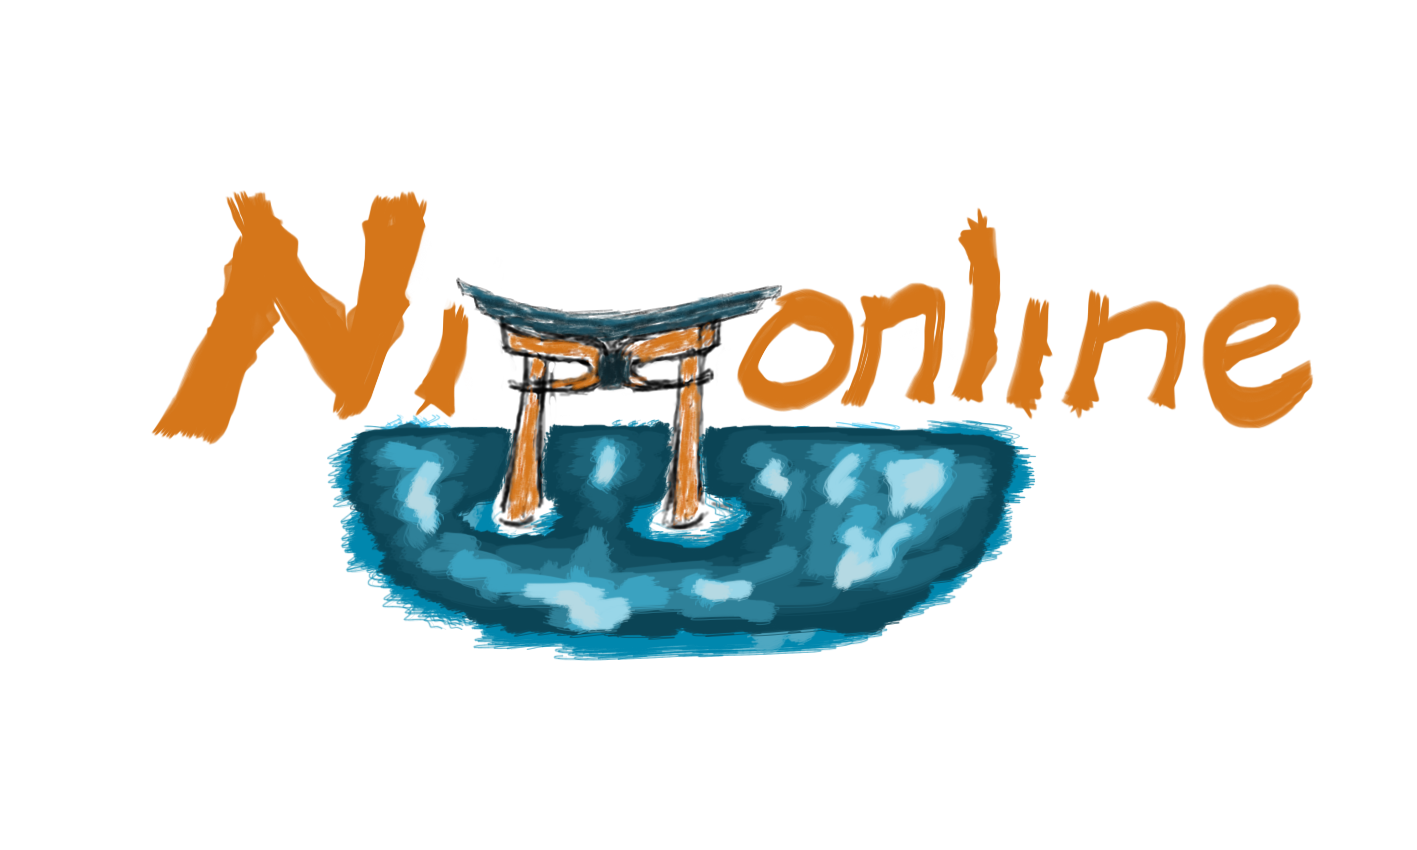
\includegraphics[width=0.7\textwidth]{nipponline_logo}

{\LARGE\Nipponline{}}

{\large{}Proyecto de Fin de Carrera}


\end{center}

\vspace{14em}
\hfill Francisco Miguel Dios Buitrago - 22222222R

\hfill Sergio Balbuena Pantigas - 9999999H

\thispagestyle{empty}
    %\include{manifiesto}
    %\include{autorizacion_biblioteca}
    \textbf{Notas aclaratorias}

'Este es un proyecto colaborativo llevado a cabo por dos estudiantes de ingenier'ia inform'atica, Francisco Miguel Dios Buitrago (FDB) y Sergio Balbuena Pantigas (SBP).

Las aplicaciones web desarrolladas en este proyecto constan b'asicamente de dos partes, la parte que se ejecuta en el navegador web del cliente (Front-end)
y la que se ejecuta en el servidor web (Back-end). Aunque no existe una clara divisi'on del trabajo, puesto que ambos alumnos han participado en la mayor'ia de tareas,
Francisco se ha enfocado m'as a la parte Back-end del proyecto (lado del servidor) mientras que Sergio se ha encargado m'as del Front-end (lado del cliente).
Por lo tanto, se han asignado las secciones de esta memoria equitativamente a ambos de ellos para poder facilitar la evaluaci'on por separado. Quedan,
sin embargo, varias secciones (introducci'on, resultados y otros) que son necesariamente comunes a ambos.

En el siguiente 'indice se especifica con sus siglas qui'en es el autor y encargado de cada secci'on, tanto en la memoria como en el proyecto. Si una secci'on no
tiene las siglas de ning'un autor, significar'a que ambos han participado y que, por lo tanto, es com'un a ambos.

Se ha elegido este modo de proceder debido a que la parte de un autor carece de sentido sin la parte del otro, por lo que para entender el proyecto
al completo es necesario tener toda la informaci'on en el mismo lugar.
    \tableofcontents
    \section{Introducci'on}
\label{sec:introduccion}


Con la reciente globalizaci'on y auge de internet, idiomas poco representados
en la poblaci'on mundial como es el caso del japon'es han ido ganando seguidores entre
los m'as j'ovenes. El inter'es en pa'ises como Jap'on, Corea o Taiw'an
ha llegado a todo el mundo gracias a series de televisi'on, m'usica, c'omics, videojuegos
y otras muchas formas de ocio.

Sin embargo, la gran diferencia entre estos idiomas y los m'as familiares como el espa'nol,
ingl'es o franc'es hace que su aprendizaje sea especialmente complicado para alguien
que no se dedique exclusivamente al estudio de dichos lenguajes. Adem'as, el hecho de que
el inter'es en estos idiomas es relativamente reciente implica que su estudio no est'e contemplado, en general, 
por academias y universidades, de forma que aquellas personas que deseen comenzar a estudiarlos
deben ser obligatoriamente autodidactas.

Si bien existen ya distintas alternativas en la red para aprender idiomas en general, incluyendo,
por ejemplo, el japon'es, todas siguen el mismo patr'on de ense'nanza para todos los idiomas
por igual, lo cual creemos que no es una soluci'on pr'actica a la hora de ense'nar lenguajes
tan distintos entre s'i.

Este proyecto propone crear un curso espec'ifico de japon'es de forma interactiva, donde
los usuarios puedan aprender el idioma desde las lecciones m'as b'asicas, como pueden ser la
escritura y la pronunciaci'on, hasta conceptos m'as complejos como la propia cultura del pa'is.


\subsection{Justificaci'on y descripci'on del proyecto}
\label{sub:justificacion_y_descripcion_del_proyecto}

Aunque hoy en d'ia ya existen cursos de japon'es online, la mayor'ia de 'estos se basan en lecciones
te'oricas donde el usuario se limita a leer y memorizar. Adem'as, muchos de estos cursos suponen
que los estudiantes ya conocen la escritura y la pronunciaci'on del idioma de antemano, centr'andose
as'i en aspectos m'as avanzados.

En este proyecto se pretende realizar un curso de idioma japon'es compuesto por un conjunto de aplicaciones
web para que los usuarios puedan aprender interactivamente en lugar de 'unicamente
leyendo teor'ia, a la vez que se entretienen. Dichas aplicaciones estar'an
agrupadas en una comunidad online donde todos los usuarios podr'an entablar relaci'on y
comparar las puntuaciones obtenidas en las aplicaciones del curso. El dise'no se har'a de tal
forma que en un futuro las aplicaciones desarrolladas puedan ser adaptadas para aprender
otros idiomas.

Hemos estado interesados en aprender este idioma desde hace varios a'nos y,
aunque hemos encontrado recursos online para aprenderlo, dichos recursos se encontraban
muy dispersos por la red: distintos sitios, distintos formatos y distintos fines. Nuestra
motivaci'on es 'esta, agrupar todo el contenido necesario para aprender el idioma en un solo
lugar y adem'as hacerlo de una forma con la que el usuario pueda aprender divirti'endose, puesto que
'esta es la mejor manera de aprender.

Pretendemos incluir elementos para dar un aire de competitividad a las aplicaciones, ya sea
mediante logros, puntuaciones, rankings u otros m'etodos para hacer que el aprendizaje del
usuario no sea totalmente en solitario, si no que pueda intercambiar experiencias con otros
usuarios. Se registrar'an datos del uso de las aplicaciones para
cada usuario por separado de forma que se pueda guiar u ofrecer consejos personalizados.

\subsection{Motivaci'on}
\label{sub:motivacion}

Este proyecto cubre los tres objetivos principales que ambos autores compart'iamos:
\begin{itemize}
 \item Aprender tecnolog'ias nuevas. Este proyecto se est'a desarrollando utilizando
 herramientas y tecnolog'ias con las que no tenemos ninguna experiencia, por el simple
 hecho de aprender cosas nuevas que puedan resultarnos 'utiles en el futuro. Por esto mismo,
 en muchas ocasiones no escogeremos el camino sencillo y directo para realizar una tarea concreta,
 si no que buscaremos una forma de hacerla que nos aporte nuevos conocimientos.
 \item Aprender nuevos idiomas. Se comenz'o este proyecto con conocimientos muy limitados del
 idioma japon'es, y poco a poco vamos aprendiendo este idioma conforme avanza el desarrollo.
 \item Crear una plataforma que resulte 'util a un n'umero elevado de personas. Como ya se ha explicado,
 en a'nos recientes los idiomas asi'aticos han ganado muchos adeptos, por lo que el p'ublico potencial
 de este proyecto es muy elevado.
\end{itemize}


\subsection{Alternativas}
\label{sub:alternativas}
Algunas de las herramientas m'as famosas que podemos encontrar por internet para aprender idiomas son las siguientes:
\begin{itemize}
 \item Busuu
 

\includegraphics[width=0.3\textwidth]{busuu}

 Permite aprender muchos idiomas, incluyendo japon'es, de forma gen'erica ( no espec'ifica para cada idioma). Es un servicio de pago.
 \item Livemocha
 
 
\includegraphics[width=0.3\textwidth]{livemocha}
 
 Como la anterior, tambi'en incluye herramientas 'utiles para aprender japon'es, pero vuelve a ser un servicio de pago.
 \item Duolingo
 
 
\includegraphics[width=0.3\textwidth]{duolingo}
 
 Presenta una forma de aprendizaje por repetici'on muy interesante, pero de momento no incluye el idioma japon'es.
 \item Kanjidamage
 
 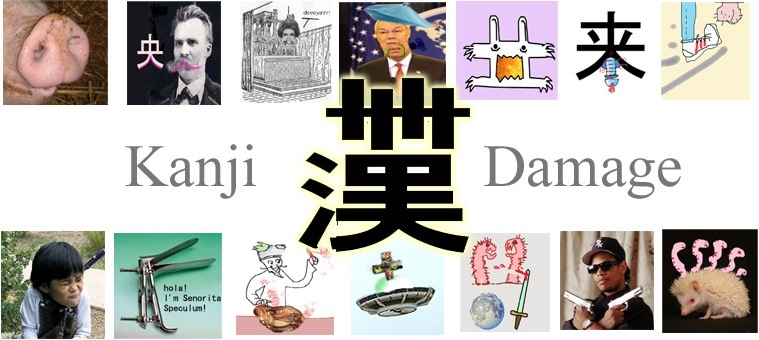
\includegraphics[width=0.3\textwidth]{kanjidamage}
 
 Aunque muy 'util, se centra exclusivamente en ense'nar una sola parte del idioma japon'es, los kanjis.
\end{itemize}


\subsection{Alcance del proyecto}
\label{sub:alcance_del_proyecto}
Como puede suponerse, la ense'nanza de un idioma al completo mediante aplicaciones interactivas no es
una tarea trivial, sobretodo teniendo en cuenta la poca experiencia de los autores tanto con el idioma
como con las tecnolog'ias utilizadas. Por lo tanto, este Proyecto de Fin de Carrera no pretende abarcar todo el
curso del idioma japon'es ni todas las caracter'isticas que deber'ia tener un curso profesional.
Este PFC se enfoca en la iniciaci'on a este idioma con aplicaciones pensadas para poder familiarizarse
con su escritura y pronunciaci'on. No obstante, este PFC es solamente el inicio de un proyecto en el que
esperamos seguir trabajando durante los pr'oximos a'nos.


    \section{Implementaci'on}
\label{sec:implementacion}


%%%%%%%%%%%%%%

\subsection{Tecnolog'ias y herramientas}
\label{sec:tecnologias_y_herramientas}

Elegir las herramientas que usar'iamos en el proyecto no fue en muchos casos una tarea sencilla. En inform'atica en general,
y en especial en el 'area de desarrollo web, aparecen cada d'ia muchas herramientas nuevas que cubren necesidades parecidas,
que solapan en cuanto a utilidad o que atacan al mismo problema desde otro punto de vista. Es por esto que
invertimos una gran parte del tiempo en estudiar las distintas tecnolog'ias disponibles para poder decantarnos por algunas
de ellas. En algunas ocasiones no hemos encontrado una herramienta claramente superior a otra, por lo que nuestra decisi'on
final se basa en cu'al nos ha llamado m'as la atenci'on o cu'al consideramos que ser'a m'as 'util en un futuro.

\subsubsection{Programaci'on front y back-end}
\label{sub:programacion_front_y_back_end}
%javascript
%nodejs

La primera elecci'on que nos tuvimos que plantear fue el lenguaje de programaci'on, puesto que esto afectar'ia considerablemente
la direcci'on que iba a tomar el proyecto. 

\begin{itemize}
\item Front-end
\begin{center}

\includegraphics[width=0.25\textwidth]{javascript}
\end{center}

Por una parte, puesto que nuestra idea era crear aplicaciones online, necesit'abamos un
lenguaje apto para ser ejecutado en un navegador web, con lo que nos dejaba con pocas opciones en el lado del cliente. Entre estas
opciones estaba Javascript, un lenguaje potente y bien documentado con una sintaxis que nos resultaba bastante familiar. Aunque existen
otras alternativas como ActionScript o Dart, nuestra decisi'on en este aspecto estaba clara. 

\item Back-end
\begin{center}

\includegraphics[width=0.4\textwidth]{nodejs}
\end{center}

Por otra parte, en cuanto a la programaci'on en el lado del servidor, nosotros ten'iamos cierta experiencia con PHP, pero lo
consider'abamos un lenguaje algo anticuado y poco llamativo, por lo que intentamos buscar otras alternativas. Dos opciones interesantes
fueron Ruby, con su framework Ruby-On-Rails, y Python con Django. A decir verdad, aunque los primeros est'an muy extendidos en el
mundo del desarrollo web, nos interesamos m'as por los segundos, que eran algo m'as novedosos y llamativos.

Sin embargo, cuando nos encontr'abamos en medio del estudio de las posibilidades que nos ofrec'ia Django, descubrimos de manera fortuita
Node.js y, aunque no era una herramienta tan madura como Ruby-On-Rails o Django, su r'apido crecimiento y algunas otras caracter'isticas
hicieron que nos decant'aramos por esta nueva opci'on sin dudarlo.

Lo que m'as nos gust'o de Node.js e hizo que nos decant'aramos por ello de inmediato es que, en el fondo, es simplemente Javascript. Un
Javascript ejecutado en el lado del servidor mediante el motor JS-V8\footnote{\url{https://developers.google.com/v8}} de Google, lo cual permite utilizar un modelo as'incrono y dirigido
por eventos que podr'a, entre otras cosas, mantener muchas conexiones al servidor abiertas y esperando sin bloquearse y consumiendo menos
recursos de la m'aquina. Adem'as, ya se han dado casos de grandes empresas que utilizan Node.js en parte de sus servicios, como es el caso de
LinkedIn, los cuales mudaron parte de su c'odigo de Ruby-On-Rails a Node.js permiti'endoles pasar de 30 a 3 servidores necesarios, entre otras
mejoras \cite{linkedin_nodejs} .

Otro punto a favor de Node.js es su gestor de paquetes NPM, con el cual se puede instalar cualquier extensi'on para back-end que exista en el repositorio
de forma r'apida y sencilla. Como se ha mencionado antes, Node.js est'a teniendo un crecimiento extremadamente r'apido, de forma que el n'umero
de m'odulos existentes para esta tecnolog'ia est'a superando a otros gigantes del sector en muy poco tiempo de vida\footnote{\url{http://modulecounts.com/}}.
Pero, sobretodo, lo m'as importante es que el tiempo que se invierte en la programaci'on de front o back-end
tambi'en nos da experiencia en la otra parte, puesto que siempre estamos usando el mismo lenguaje.

\item Aplicaciones m'oviles
\begin{center}

\includegraphics[width=0.4\textwidth]{phonegap}
\end{center}

Con el reciente auge del smartphone no se pod'ia pasar por alto el hecho de que si nuestras aplicaciones no llegan a dispositivos m'oviles
estar'iamos perdiendo una gran parte del p'ublico potencial. Es por esto que, aunque en este PFC no hemos desarrollado nada centrado en
este tema, s'i que hemos buscado qu'e posibilidades exist'ian para solventar este problema. Siguiendo la misma filosof'ia mostrada en las
secciones anteriores, encontramos una herramienta llamada PhoneGap\footnote{\url{http://phonegap.com}} que permite crear aplicaciones m'oviles usando simplemente Javascript y
HTML5, sin necesidad de invertir tiempo en aprender tecnolog'ias especializadas para cada plataforma m'ovil, como Android, iOS o Windows Phone.

Encontramos, en definitiva, una raz'on m'as para elegir Javascript como piedra angular del proyecto.


\end{itemize}


\subsubsection{Web Application Framework}
\label{sub:web_application_framework}
%expressjs
Es aconsejable el uso de un back-end web framework para facilitar la creaci'on de aplicaciones web. Aunque se puede utilizar Node.js sin m'as,
esto nos obligar'ia a tener que implementar muchas tareas repetibles que ya han sido solucionadas y optimizadas en estos frameworks web.

\begin{center}

\includegraphics[width=0.5\textwidth]{express}
\end{center}

El rey por excelencia en este 'ambito es Express.js, el cual ayudar'a en la organizaci'on de las aplicaciones web ofreciendo una arquitectura
Model-View-Controller. Adem'as, se encargar'a de las rutas de la aplicaci'on, de las peticiones a la base de datos, gesti'on de cookies,
facilidades con motores de plantilla como Jade o Handlebars y de otras muchas caracter'isticas.

\subsubsection{Boilerplate}
\label{sub:boilerplate}

\subsubsection{Base de datos}
\label{sub:base_de_datos}
%mongodb
%mongoose

\subsubsection{Configuraci'on del servidor}
\label{sub:configuracion_del_servidor}
%nginx

\subsubsection{Comunicaci'on cliente-servidor}
\label{sub:comunicacion_cliente_servidor}
%socket.io

\Nipponline{} es un proyecto de software libre y c'odigo abierto, por lo que cualquiera puede unirse al proyecto y
colaborar con 'este desarrollando nuevas funcionalidades para el mismo.

Uno de los principales elementos del proyecto son las aplicaciones del lado del cliente enfocadas a aprender
japon'es, y de las cuales tambi'en queremos que nuestros futuros colaboradores puedan ser part'icipes, de forma que
puedan desarrollar libremente nuevas aplicaciones que diferentes a las ya existentes por su cuenta.

A fin de lograr este objetivo hemos trabajado (y seguimos trabajando) en ofrecer desde el servidor una API con
diferentes llamadas, para realizar diferentes tareas como obtener y enviar datos al servidor, que facilitar'an la
tarea a nuevos colaboradores y desarrolladores que quieran trabajar en sus propias aplicaciones, sin tener que
entretenerse en leer toda la documentaci'on e implementaci'on del lado del servidor del proyecto.

Para esta tarea hemos utilizado la tecnolog'ia Socket.IO\footnote{\url{http://socket.io/}}. Socket.IO es una 
biblioteca para Javascript orientada a eventos que permite una comunicaci'on bidireccional y en tiempo real 
entre clientes y el servidor. Como se ilustra en la siguiente figura, Socket.IO se compone de dos librer'ias, una se 
ejecuta en el lado del servidor con Node.js, mientras que la otra se encuentra en el lado del cliente.

\begin{center}
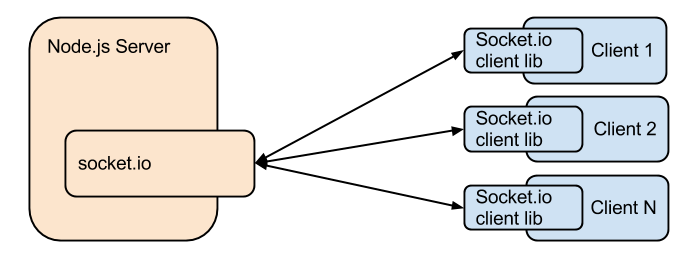
\includegraphics[width=0.7\textwidth]{socketio}
\end{center}

En el servidor se configuran los diferentes callback que deben invocarse como resultado de las llamadas Socket.IO
realizadas por el cliente, de forma que extraigan los datos enviados (si se enviaron datos), realicen las acciones
necesarias (extracci'on o almacenamiento en la base de datos, por ejemplo) y devuelvan una confirmaci'on al cliente
(con datos adicionales, si es necesario).

Desde el cliente basta con importar la biblioteca de Socket.IO del cliente y establecer una conexi'on con el servidor:

\begin{verbatim}
var socket = io.connect();
\end{verbatim}

Al realizar la conexi'on inicial, el servidor siempre env'ia una respuesta al cliente notific'andole si tiene una
sesi'on abierta o no con el servidor (True o False). Desde el cliente es posible capturar esta respuesta:

\begin{verbatim}
socket.on('acknowledge', function(data){
    console.log(data);
});
\end{verbatim}

En el c'odigo anterior simplemente se define una funci'on de callback que se ejecutar'a al recibir del servidor un
mensaje marcado como 'acknowledge'. El argumento data de la funci'on es donde se encontrar'an los datos devueltos
por el servidor (si se devuelven datos).

\subsubsection{Biblioteca de dibujo}
\label{sub:biblioteca_de_dibujo}
%createjs

Como ya hemos comentado anteriormente, nuestro lenguaje de elecci'on para la programaci'on en el
lado del cliente va a ser Javascript. 
Uno de los principales elementos de \Nipponline{} son las aplicaciones del cliente, que permiten a
los usuarios aprender y reforzar su conocimiento del idioma japon'es a trav'es de minijuegos. El
alto componente de gr'aficos y animaciones de estos minijuegos nos plantea un nuevo problema, ya
que no podemos limitarnos a usar simplemente Javascript. Debemos, adem'as, hacer uso de una
biblioteca o framework que nos ayude en la tarea de programar los juegos para el cliente en
Javascript.

Nuestra elecci'on para esta tarea es CreateJS\footnote{\url{http://www.createjs.com/}}, una suite compuesta de 4 
sub-frameworks que a'naden funcionalidad a Javascript, facilitando el desarrollo de aplicaciones
gr'aficas e interactivas mediante el dibujado en elementos canvas (lienzo) de HTML.

\begin{center}
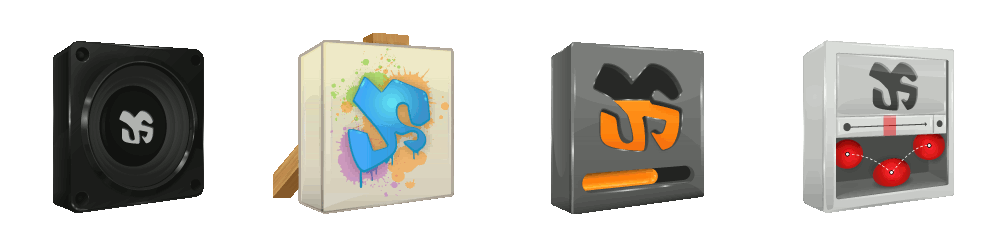
\includegraphics[width=0.8\textwidth]{create_suite}
\end{center}

Los 4 sub-frameworks de CreateJS mencionados son:

\begin{itemize}
\item \textbf{EaselJS.} Probablemente el componente m'as importante de la suite, ya que es el que incluye
toda la funcionalidad necesaria para dibujar en el canvas, as'i como crear y manejar animaciones
personalizadas.
\item \textbf{TweenJS.} Tween (o Inbetweening) consiste en animar un elemento de forma que una (o varias)
de sus propiedades evolucionen de forma m'as o menos suave en el tiempo. Esto permite realizar
animaciones de car'acter m'as general de forma autom'atica (sin usar c'odigo espec'ifico de 
control en el bucle de animaci'on), como puede ser desplazar o escalar una imagen en el tiempo.
\item \textbf{SoundJS.} Este componente es el que, como su nombre indica, permite el uso de sonido en las
aplicaciones.
\item \textbf{PreloadJS.} Este componente permite realizar la carga de recursos (im'agenes o sonidos) desde
el servidor de forma automatizada y as'incrona, proporcionando la posibilidad de definir callbacks
para su coordinaci'on.
\end{itemize}

Los principales motivos de decidirnos por el uso de la suite de CreateJS se enumeran a continuaci'on:

\begin{itemize}
\item \textbf{Estilo de programaci'on.} Despu'es de examinar la API y las demos que ofrecidas por la 
comunidad de CreateJS comprobamos que el estilo de uso de las funciones para dibujado y animaci'on
es bastante similar al que est'abamos acostumbrados a utilizar en otros proyectos en los que 
hemos trabajado con gr'aficos.
\item \textbf{Licencia.} CreateJS est'a sujeto a una licencia MIT, por lo que se adapta perfectamente a 
nuestras necesidades de uso exclusivo de software libre. Adem'as, si fuese necesario, la licencia
MIT nos permite realizar modificaciones sin necesidad de aplicar nuevamente una licencia MIT al 
resultado.
\end{itemize}

A continuaci'on se mencionan varias alternativas para dibujado en el lado del cliente que se han
considerado, pero que finalmente no hemos usado:

\begin{itemize}
\item \textbf{gameQuery\footnote{\url{http://gamequeryjs.com/}}.} Extensi'on para jQuery que facilita la realizaci'on 
de animaciones y juegos en general. Su uso fue descartado debido a que se basaba en la manipulaci'on
del DOM, en lugar de usar elementos canvas de HTML (dibujando sobre estos). 
La justificaci'on de esta decisi'on est'a en el hecho de que nuestra poca experiencia en
desarrollo web nos hac'ia reticentes a jugar con el DOM. Por otra parte, usando una biblioteca
de dibujado en el canvas pod'iamos despreocuparnos de  la manipulaci'on del DOM y centrarnos
'unicamente en lo que ocurre dentro del canvas.
Para finalizar, tambi'en hemos tenido en cuenta que el dibujado sobre el canvas es ligeramente
m'as eficiente en la mayor'ia de los casos que manipular el DOM, adem'as de ofrecer una mayor
compatibilidad entre navegadores web.

\begin{center}

\includegraphics[width=0.4\textwidth]{gamequery}
\end{center}

\item \textbf{LimeJS\footnote{\url{http://www.limejs.com/}}.} Otra biblioteca para gr'aficos con Javascript con funcionalidad similar a la 
ofrecida por CreateJS. Sin embargo, LimeJS no proporciona una utilidad de precarga de recursos 
(a diferencia de CreateJS, que proporciona PreloadJS), por lo que deber'iamos implementar algo
similar por nuestra cuenta o buscar alguna alternativa. Adem'as, LimeJS requiere tener Python
instalado para su uso, lo que impone unas restricciones adicionales a los desarrolladores.
\item \textbf{MelonJS\footnote{\url{http://melonjs.org/}}.} Una alternativa m'as que, al igual que LimeJS, ofrece una funcionalidad muy similar
a la de CreateJS. Del mismo modo, el motivo por el cual esta biblioteca no ha sido usada es la 
ausencia de un m'odulo para el precargado de recursos que CreateJS s'i ofrece.
\item \textbf{GameMaker\footnote{\url{https://www.yoyogames.com/studio}}.} Una biblioteca potente con multitud de funcionalidades. Desafortunadamente, su
licencia es de pago y, por tanto, incompatible con nuestro proyecto (que pretende ser un proyecto
de software libre que utiliza 'unicamente elementos de la misma naturaleza), motivo por el cual 
es desechada.
\end{itemize}

\subsubsection{Internacionalizaci'on}
\label{sub:internacionalizacion}
%i18n

Dado que queremos abrir el uso de nuestras aplicaciones a la mayor cantidad de p'ublico posible necesitamos
asegurarnos de su traducci'on a varios idiomas. A la hora de traducir una aplicaci'on hay dos elementos a tener en
cuenta: la internacionalizaci'on (i18n) y la localizaci'on (l10n) de la aplicaci'on.

\begin{itemize}
\item \textbf{Internacionalizaci'on.} Consiste en el dise'no de software (en nuestro caso las aplicaciones) de forma
que sea posible su traducci'on a diferentes idiomas sin que ello conlleve realizar modificaciones en el
c'odigo/dise'no de este.
\item \textbf{Localizaci'on.} Se trata de la traducci'on de la aplicaci'on a un idioma concreto en s'i. Se sirve de
los mecanismos proporcionados por la internacionalizaci'on para mostrar la traducci'on.
\end{itemize}

Podemos deducir f'acilmente que la fase de internacionalizaci'on es la m'as compleja desde el punto de visto del
dise'no y desarrollo de nuestras aplicaciones. Debemos plantearnos cuestiones tales como la forma en que la
aplicaci'on detecta las preferencias de idioma de los usuarios, c'omo almacenar en el servidor las traducciones
correspondientes, con qu'e formato, etc.

Nosotros hemos decidido hacer uso de la biblioteca i18next\footnote{\url{http://i18next.com/}}, compatible con 
Javascript y Node.js. Esta biblioteca se basa en la existencia de un directorio de 'locales' en el servidor, donde 
se almacenan las traducciones de diferentes textos de las aplicaciones en formato JSON. Al iniciar el servidor, se 
inicializa i18next, indic'andole donde se encuentra el directorio de 'locales':

\begin{verbatim}
i18n.init({
    resGetPath: 'public/locales/__lng__/__ns__.json'
});
\end{verbatim}

A partir de este momento, las peticiones de clientes de traducciones har'an que el servidor env'ie el archivo JSON
correspondiente al idioma indicado por el cliente (existe un directorio por defecto en ingl'es que se usa cuando el
idioma del cliente no est'a disponible).

El Javascript del cliente, por su parte,  debe importar la biblioteca i18next e inicializar la variable i18n para
recibir la traducci'on del servidor:

\begin{verbatim}
i18n.init({ useCookie: false }, callback);
\end{verbatim}

Como se puede ver, es posible asignar una funci'on de callback que es llamada en cuanto se recibe el JSON del
servidor y cuyo cometido suele ser realizar la traducci'on de la aplicaci'on del cliente.
Por defecto, i18next toma el idioma favorito del navegador para realizar la petici'on del archivo JSON con las
traducciones al servidor, aunque es posible indicar un idioma concreto.

Una vez recibido el JSON con las traducciones, acceder a estas solo requiere conocer la etiqueta de la traducci'on
concreta que se quiere obtener:

\begin{verbatim}
translation = i18n.t("textField1");
\end{verbatim}

\subsubsection{Gamificaci'on}
\label{sub:gamificacion}
%mozillaBadges

Como ya hemos comentado, con \Nipponline{} no queremos limitarnos solo al desarrollo de un conjunto de aplicaciones para
aprender japon'es, sino que adem'as queremos crear una comunidad donde diferentes usuarios puedan interactuar entre
s'i.

El primer paso en la creaci'on de la comunidad pasa por el uso de unos foros que en nuestro caso nos proporciona un
software de terceros. 
Adicionalmente, queremos a'nadir a \Nipponline{} una Gaming Layer: los usuarios de \Nipponline{} tendr'an niveles, objetos
o logros asociados a su cuenta. Todos estos elementos ser'an desbloqueables por medio de la participaci'on en la
comunidad (participando en los foros, usando las aplicaciones y/o obteniendo ciertas puntuaciones en estas).

Para implementar, en parte, esta funcionalidad nos hemos decantado por el uso de las OpenBadges de 
Mozilla\footnote{\url{http://www.openbadges.org/}}.

\begin{center}

\includegraphics[width=0.5\textwidth]{mozilla_badges}
\end{center}

OpenBadges permite a sitios web (como \Nipponline{}) definir un conjunto de badges (medallas o insignias) a ser 
obtenidas por los usuarios de dichos sitios web al completar ciertas tareas. Estas insignias se almacenan en la
Mozilla Backpack del usuario, que puede a partir de ese momento mostrar sus nuevas insignias en cualquier sitio web
que implemente la capacidad de mostrar OpenBadges. 

En la siguiente figura se ilustra la infraestructura\cite{mozillawiki}  y funcionamiento abstracto de 
OpenBadges.

\begin{center}
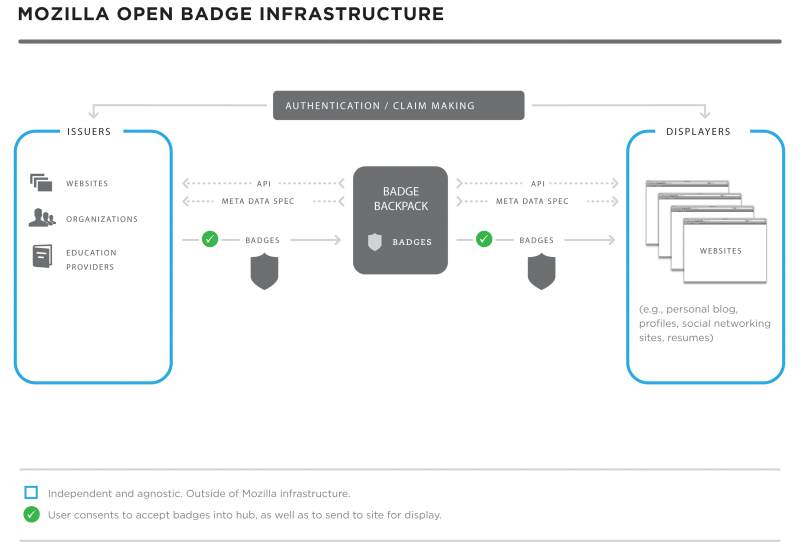
\includegraphics[width=1.0\textwidth]{badges_infrastructure}
\end{center}

OpenBadges es software libre, al igual que \Nipponline{}, con las ventajas que esto conlleva. Cualquiera puede crear y
otorgar su propio conjunto de insignias a usuarios por realizar tareas.
Adem'as, los usuarios pueden mostrar, si as'i lo desean, las insignias obtenidas en \Nipponline{} en cualquier lugar en
el que esto sea posible (existen plugins para Wordpress o Twitter que a'naden esta  funcionalidad). Esta es la raz'on
principal de hacer uso de OpenBadges en \Nipponline{} en lugar de crear nuestro propio conjunto de insignias privado
(caso en el que las insignias obtenidas no habr'ian abandonado el 'ambito de \Nipponline{}, limitando la difusi'on de la
comunidad).

Una desventaja del uso de OpenBadges es el hecho de que es necesario que el usuario posea una Mozilla Backpack donde
almacenar las insignias, aunque si no posee una puede optar por no obtener la insignia sin que ello supongo problema
alguno. 

\subsubsection{Control de versiones}
\label{sub:control_de_versiones}
%Git
%Github

Dada la naturaleza colaborativa del proyecto \Nipponline{} (no solo hemos trabajado conjuntamente en 'el dos personas, 
sino que al ser software libre es posible que en el futuro aparezcan nuevos colaboradores para trabajar en el 
proyecto) necesitamos utilizar alg'un software de control de versiones que permita la colaboraci'on fluida y de forma
sencilla de diferentes personas en el desarrollo del proyecto.

Obviamente, es imposible trabajar en el proyecto de forma local, dado que desde un primer momento hemos sido personas
los que hemos estado trabajando en el desarrollo de \Nipponline{}. Adem'as, conforme un proyecto va creciendo se hace
cada vez m'as dif'icil mantener de forma local el historial de cambios del mismo y su mantenimiento se vuelve muy
tedioso.

As'i pues, queda claro que debemos usar alguna herramienta para el control de versiones. En este punto debemos
decidir si vamos a emplear un sistema de control de versiones centralizado o distribuido, as'i como la herramienta
concreta a usar.

A continuaci'on se comentan los dos tipos de sistemas de control de versiones\cite{versioncontrol} considerados y el
motivo de elegir uno sobre el otro.

\begin{itemize}
\item \textbf{Control de versiones centralizado:} En este esquema existe un 'unico repositorio central y todos los
cambios realizados en el proyecto por parte de los colaboradores deben ser enviados a este repositorio. Obviamente,
para poder realizar cambios en el proyecto es necesario que los colaboradores se descarguen los 'ultimos cambios
realizados por otros usuarios y que pueden no estar actualizados en su copia local del proyecto.
Algunas conocidas herramientas de control de versiones centralizado son SVN y CVS.

\begin{center}
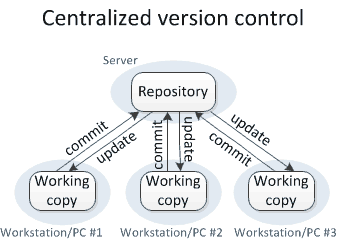
\includegraphics[width=0.7\textwidth]{version_centralized}
\end{center}

\item \textbf{Control de versiones distribuido:} En este esquema no existe un 'unico repositorio, sino que cada
colaborador del proyecto obtiene su propio repositorio sobre el que puede trabajar de forma independiente sin
necesidad de actualizarlo con los cambios que realicen otros usuarios. Cabe destacar que el hecho de que no exista
un 'unico repositorio no implica necesariamente que no haya un repositorio maestro en el que converjan los cambios
realizados por todos los colaboradores.
Entre las herramientas de control de versiones distribuido se encuentran Git, Mercurial y Bazaar.

\begin{center}
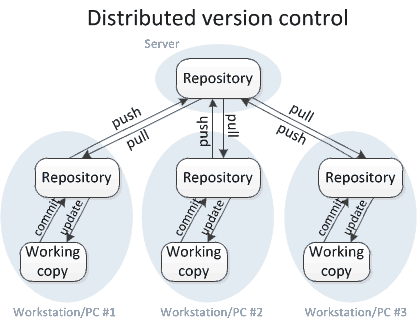
\includegraphics[width=0.7\textwidth]{version_distributed}
\end{center}

\end{itemize}

Vemos pues que frente al control de versiones centralizado, un esquema distribuido aporta pr'acticamente solo mejoras
y una mayor flexibilidad durante el desarrollo del proyecto, motivo por el cual nos decidimos claramente por el uso
de un sistema de control de versiones distribuido.

\textbf{Git}

Entre las diferentes alternativas disponibles para control de versiones distribuido nos hemos decantado por Git.
A continuaci'on se resumen algunas de las caracter'isticas de Git\footnote{\url{http://git-scm.com/about/}}.

\begin{itemize}
\item \textbf{Licencia GPL.} Git es software libre y de c'odigo abierto, por lo que cualquiera puede modificarlo de
la forma que considere oportuna.
\item \textbf{Rapidez.} Git es r'apido en sistemas Linux, incluso m'as que otras herramientas de control de versiones
distribuidas como Mercurial. El hecho de ser distribuido le da una gran ventaja en velocidad sobre otras herramientas
de control de versiones centralizadas, ya que todas las operaciones se hacen de forma local, mientras que en los
sistemas centralizados es necesario comunicarse con el servidor donde se encuentra el repositorio para cada
operaci'on.
\item \textbf{Modelo de ramas.} Una de las caracter'isticas m'as reconocibles de Git es la posibilidad de trabajar
con ramas, copias del repositorio original sobre las que se puede trabajar de forma independiente para probar cosas
nuevas o arriesgadas cuyo impacto en el proyecto es desconocido o se quiere medir, sin que estos cambios afecten a
la rama principal del proyecto. Una vez finalizado el trabajo sobre la rama es posible fusionarla con la rama
principal o descartar los cambios realizados en funci'on del resultado de estos.
\item \textbf{'indice.} Todos los proyectos usando Git usan un 'indice o staging area que permite configurar los
commit o cambios del repositorio de forma flexible. Es posible, por ejemplo, actualizar en el repositorio con un
commit solo algunos ficheros de todos los modificados o diferentes cambios consecutivos sobre un mismo fichero en
diferentes commits.

\begin{center}
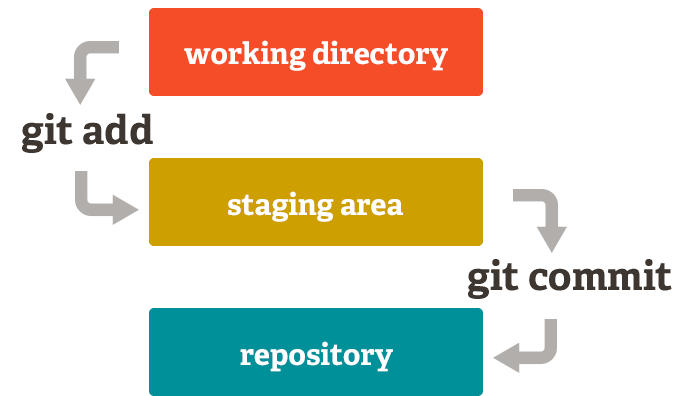
\includegraphics[width=0.6\textwidth]{index}
\end{center}

\item \textbf{Seguridad e integridad de los datos.} Git utiliza sumas de verificaci'on (checksums) en todos los
ficheros y commits de un proyecto, lo que permite tener un control total de los cambios del mismo, impidiendo que
cambios externos el sistema de control de versiones pasen inadvertidos a este.
\item \textbf{Apoyo.} Git es una de las herramientas de control de versiones con mayor apoyo en forma de n'umero de
plataformas de hosting (GitHub, Google Code) que soportan su uso, frente a otras como Mercurial que cuentan con un
apoyo menor.
\end{itemize}

\textbf{GitHub}

Finalmente, una vez escogido nuestro sistema de control de versiones nos queda escoger una plataforma a trav'es de la
cual podamos distribuir nuestro proyecto y que soporte el uso de Git. Hemos elegido para ello GitHub, por ser una
comunidad muy activa de desarrolladores, que alberga numerosos proyectos de distinta envergadura.

GitHub permite tener un n'umero ilimitado de repositorios p'ublicos y requiere una suscripci'on de pago para poder
crear repositorios privados. No obstante, dado que nuestro proyecto es de c'odigo libre, vamos a crear un repositorio
p'ublico y nos supone ning'un obst'aculo la limitaci'on en cuanto a repositorios privados.

Otra caracter'istica interesante de GitHub es el hecho de permitir un n'umero ilimitado de colaboradores en los
repositorios, algo que otras plataformas no permiten. Esto permite que al proyecto puedan adherirse tantos
colaboradores como haga falta si en el futuro este ganara suficiente popularidad.

%%%%%%%%%%%%%%

\subsection{Comunidad}
\label{sec:comunidad}

%%%%%%%%%%%%%%

\subsection{Aplicaciones}
\label{sec:aplicaciones}

Las aplicaciones desarrolladas comparten una serie de elementos y estructura. Los principales 
elementos comunes se listan a continuaci'on:

\begin{itemize}
\item \textbf{Comunicaci'on con el servidor.} La comunicaci'on con el servidor se realiza con la ayuda de la interfaz 
Socket.IO. El tipo de peticiones enviadas al servidor var'ia en funci'on de la aplicaci'on concreta (por ejemplo, el
minijuego-1 pide al servidor que le env'ie una lista con las diferentes s'ilabas del lenguaje japon'es, mientras que
el minijuego-2 pide una lista de palabras).
Tambi'en es por medio de Socket.IO que las aplicaciones son capaces de detectar si el usuario tiene una sesi'on 
iniciada, en cuyo caso sus estad'isticas son enviadas y registradas en el servidor.
\item \textbf{Estructura HTML.} Todas las aplicaciones comparten una misma estructura HTML cuyo punto central es un elemento
canvas sobre el que se realiza el dibujado necesario, as'i como una pantalla de carga (creada con elementos div y 
CSS) que solo es visible mientras se cargan los recursos de la aplicaci'on concreta.
Al margen de estos elementos, cada aplicaci'on incluye una serie de elementos propios como pueden ser campos de texto
o botones, en funci'on de las necesidades de la misma.
\item \textbf{Precarga de recursos.} Con la ayuda de la biblioteca PreloadJS ofrecida por CreateJS es posible declarar una
lista personalizada con todos los recursos necesarios para la aplicaci'on (im'agenes o audio) y enviar una petici'on
al servidor para que nos devuelva estos recursos.
PreloadJS ofrece adem'as funciones callback que se invocan durante el proceso de precarga cada vez que este avanza,
lo que nos permite, haciendo uso de jQuery, actualizar la pantalla de carga y borrarla una vez se ha completado la
carga.
Para realizar la carga debemos declarar primero una lista de objetos JSON que contenga todos los recursos que 
queremos que el servidor nos env'ie.

\begin{verbatim}
manifest = [];
manifest.push({src:"images/app2/bg.png", id:"bg", 
                 imageType:"background"});
manifest.push({src:"images/app2/power1.gif", id:"power1"});
\end{verbatim}

el atributo 'src' es obligatorio e indica al servidor la ruta, dentro del directorio public, que ocupa el archivo
a traer en el servidor, mientras que el atributo 'id' se utiliza para identificar el recurso en concreto. El atributo
imageType se utiliza para tratar de forma diferente a las im'agenes seg'un sean spritesheets, backgrounds (fondos)
o im'agenes normales.

Una vez declarado el manifiesto debemos cargarlo para que PreloadJS se encargue de hacer las peticiones 
correspondientes al servidor. Adicionalmente definimos varias funciones de callback:

\begin{verbatim}
queue = new createjs.LoadQueue();
queue.addEventListener("progress", handleProgress);
queue.addEventListener("complete", handleComplete);
queue.addEventListener("fileload", handleFileLoad);
queue.loadManifest(manifest);
\end{verbatim}

El evento 'progress' tiene lugar cada cierto porcentaje del proceso de carga, y se utiliza el callback asociado a 
este evento, la funci'on handleProgress, para modificar y hacer avanzar la barra de progreso en la pantalla de carga
de la aplicaci'on.
El evento 'fileload' ocurre cada vez que se termina de cargar un archivo del manifiesto y su callback se encarga de
tratar cada uno de los archivos de la forma indicada. As'i, por ejemplo, una imagen de tipo spritesheet es procesada 
para crear un objeto de animaci'on Sprite de EaselJS.
El evento 'complete' solo tiene lugar una vez, al terminar de cargar todos los recursos. Su callback, handleComplete,
se encarga de ocultar la pantalla de carga y dejar la aplicaci'on en su estado inicial.
\item \textbf{Internacionalizaci'on.} Todas las aplicaciones hacen uso de la biblioteca i18next, para internacionalizaci'on
con Javascript. El uso de la biblioteca es simple, basta con hacer una llamada de inicializaci'on al inicio de la
aplicaci'on para que el servidor nos env'ie el archivo de localizaci'on correspondiente. Una vez hemos recibido el
resultado (es posible definir una funci'on de callback para cuando se reciba la respuesta del servidor), tenemos 
acceso a las traducciones de los diferentes texto de la aplicaci'on a trav'es de un objeto JSON.
\item \textbf{Bucle de animaci'on.} Las aplicaciones implementan una funci'on update() que gestiona todo el bucle de 
animaci'on y que es llamada FPS veces por segundo, donde FPS (frames per second) suele ser 30 y se refiere al n'umero
de refrescos de pantalla por segundo.
La funci'on update se puede descomponer en 3 fases, ilustradas a continuaci'on:

\begin{center}
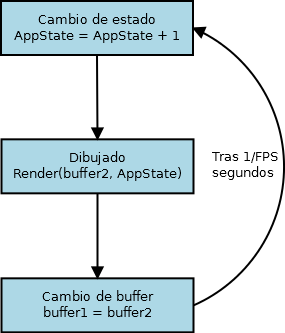
\includegraphics[width=0.4\textwidth]{draw2d}
\end{center}

\begin{enumerate}
\item \textbf{Cambio de estado.} En esta fase se llevan a cabo todas las tareas relativas a la l'ogica de aplicaci'on,
pasando de un estado de la aplicaci'on dado (el actual) al siguiente en funci'on del mismo. As'i, se realizan tareas
como cambiar la posici'on de elementos en la pantalla seg'un la velocidad que lleven o disminuir la cantidad de 
energ'ia del jugador si se detecta una colisi'on del mismo con un elemento da'nino.
\item \textbf{Dibujado.} Una vez obtenido el nuevo estado de la aplicaci'on debemos dibujarlo en el lienzo para sustituir
al antiguo, de forma que el usuario aprecie en pantalla los cambios que van sucediendo en la aplicaci'on.
\item \textbf{Cambio de buffer.} Generalmente se utiliza una t'ecnica de doble buffer para dibujar en pantalla. Esta
t'ecnica consiste en realizar la fase 2 (dibujado) sobre un buffer, en lugar de sobre la pantalla directamente, lo 
cual podr'ia ocasionar un efecto de parpadeo. Una vez se ha dibujado sobre el buffer oculto, se sustituyen los 
contenidos de la pantalla por los del buffer.
En la siguiente figura se ilustra el funcionamiento del cambio de buffer.


\centerline{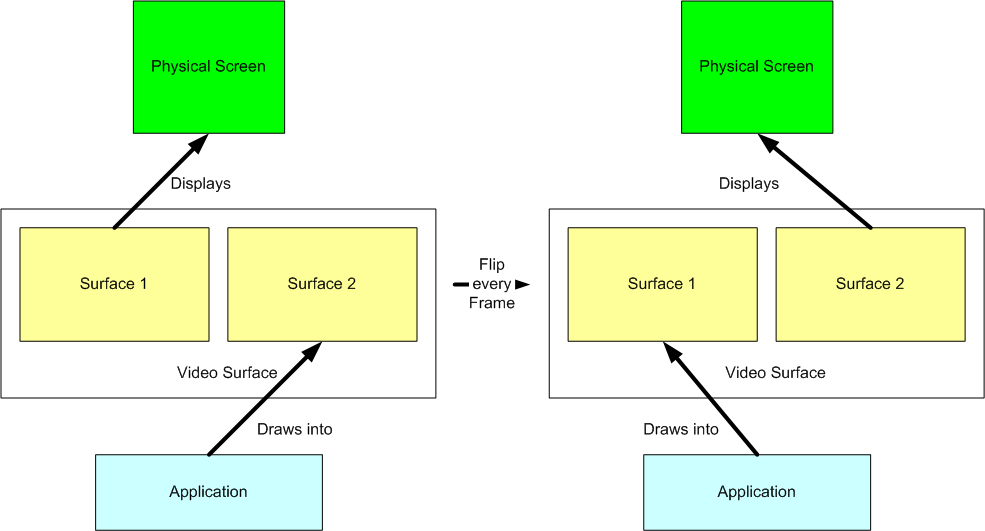
\includegraphics[width=1.1\textwidth]{double_buffer}}

En nuestras aplicaciones, no obstante, solo diferenciamos 2 fases, ya que CreateJS abstrae las fases 2 y 3 en una
'unica funci'on de actualizaci'on del canvas.
\end{enumerate}
\end{itemize}

\subsubsection{Syllables}
\label{sub:syllables}

El objetivo de esta aplicaci'on es el de introducir al usuario al lenguaje japon'es por medio de la pr'actica y
aprendizaje de los diferentes silabarios de los que est'a compuesto el lenguaje.

\begin{center}
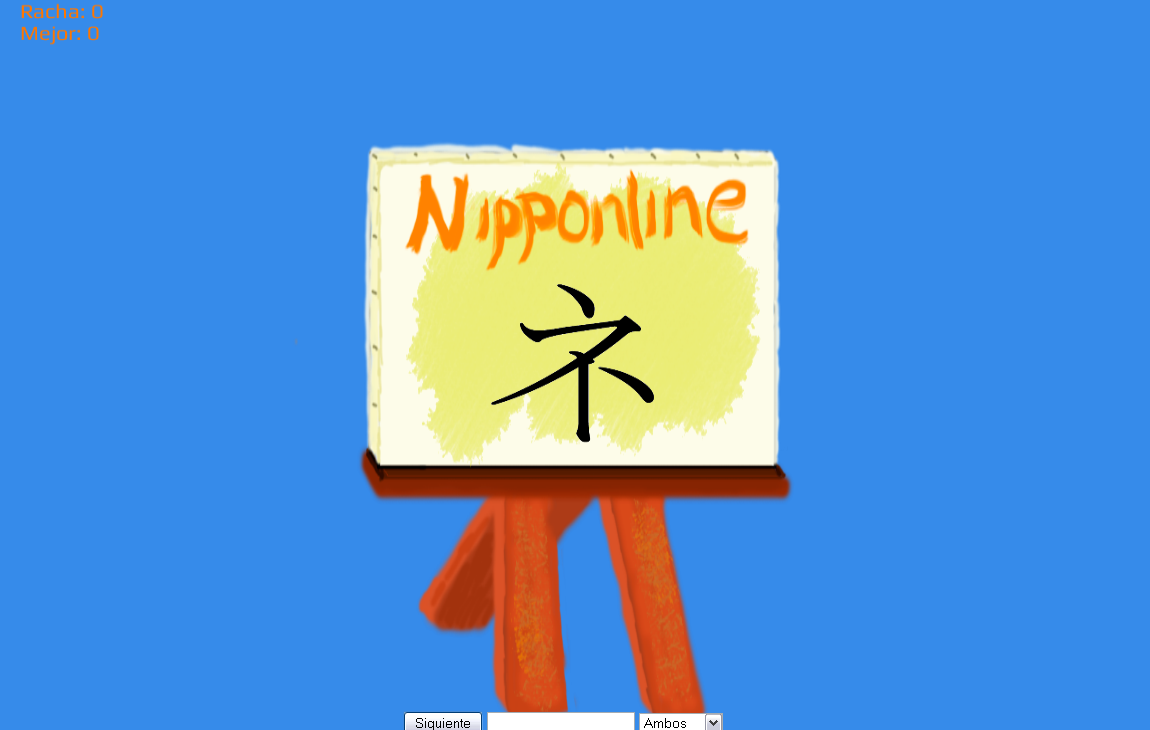
\includegraphics[width=0.8\textwidth]{syllables_capt}
\end{center}

\textbf{Interfaz y funcionamiento}

En esta aplicaci'on se le presenta al usuario un lienzo sobre el que se dibujan s'ilabas japonesas (denominadas kana).
El objetivo del usuario es el de escribir en el campo de texto que se le proporciona la correspondiente romanizaci'on
(escritura en alfabeto latino) de las s'ilabas mostradas en pantalla.

La interfaz incluye un bot'on para pasar a la siguiente s'ilaba (contando la s'ilaba actual como fallo) en caso de 
que el usuario sea incapaz de reconocer la s'ilaba en pantalla, as'i como una lista desplegable que le permite elegir
a qu'e silabario pertenecer'an las s'ilabas mostradas en el futuro.

La aplicaci'on mantiene un recuento de las estad'isticas del usuario en forma del n'umero de s'ilabas consecutivas
que es capaz de acertar, as'i como la cantidad de veces que ha acertado  o fallado una cierta s'ilaba y el tiempo
medio empleado en cada cierto. El servidor recibe con cierta regularidad actualizaciones de estas estad'isticas
conforme el usuario utiliza la aplicaci'on a fin de mantenerlas actualizadas en la base de datos.

\textbf{Implementaci'on}

\begin{itemize}
\item \textbf{Petici'on al servidor.} La aplicaci'on comienza haciendo una petici'on al servidor del conjunto de todas las 
s'ilabas por medio de la API con Socket.IO:

\begin{verbatim}
socket.emit('getsyllables', 0, function (data) {
    kana = data;
});
\end{verbatim}

Tambi'en se define una funci'on de callback que se ejecuta en cuanto se obtiene la respuesta del servidor para asignar
el conjunto de s'ilabas obtenido a una variable local de la aplicaci'on.
\item \textbf{Interacci'on con el usuario.} El HTML de la aplicaci'on incluye un campo de texto en el que el usuario puede
escribir la romanizaci'on de las diferentes s'ilabas que aparecen en pantalla. Cambios en la entrada del campo de
texto se monitorizan a fin de comprobar si el usuario ha escrito la s'ilaba correctamente.
Tambi'en se han asociado funciones de respuesta a la pulsaci'on del bot'on para pasar de s'ilaba (se escoge una nueva
s'ilaba al azar para sustituir a la actual) y al cambio de opci'on en el men'u desplegable (se restringe el conjunto
de s'ilabas que pueden aparecer en pantalla en funci'on de la opci'on seleccionada).
\item \textbf{Actualizaci'on de estad'isticas.} Como ya hemos comentado, cada cierto tiempo se env'ia al servidor una 
actualizaci'on con las 'ultimas estad'isticas del usuario. Para ello vamos a utilizar la API con Socket.IO para 
comunicarnos con el servidor, como hicimos para obtener el conjunto de s'ilabas al inicio de la aplicaci'on.

\begin{verbatim}
socket.emit('game1:stats', [stats, streak], function (){
    // Respuesta del servidor
});
\end{verbatim}

En este caso vamos a enviar informaci'on al servidor, para lo cual usamos el segundo argumento de socket.emit, donde
depositamos las estad'isticas del usuario en esta aplicaci'on.
Obviamente, no es posible enviarle cualquier cosa al servidor, ya que este realiza las comprobaciones adecuadas al
recibir los datos para validarlos y comprobar que se ajustan al formato espec'ifico y que son realistas.
\end{itemize}

\subsubsection{Words}
\label{sub:words}

Esta aplicaci'on tiene como objetivo reforzar y profundizar en la pr'actica del usuario con los silabarios japoneses,
para lo cual propone al usuario escribir la romanizaci'on correspondiente a las palabras que aparecen en pantalla
(escritas con sus correspondientes kana).

\begin{center}
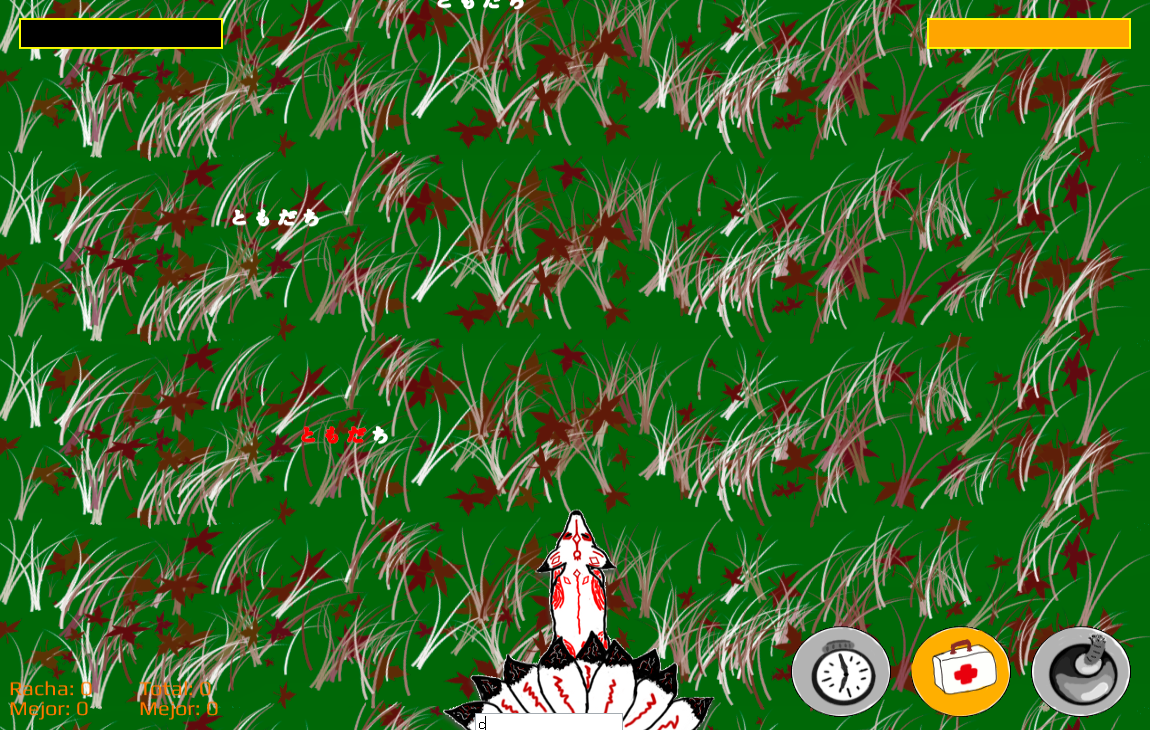
\includegraphics[width=0.8\textwidth]{okami_capt}
\end{center}

\textbf{Interfaz y funcionamiento}

En esta aplicaci'on el usuario est'a representado por un zorro que se desplaza por un campo. Desde la parte superior
de la pantalla aparecen palabras en japon'es cuya romanizaci'on debe escribir el usuario, de modo que desaparezcan
antes de que entren en contacto con su avatar (el zorro), lo cual provocar'ia que perdiera puntos de vitalidad (PV
de ahora en adelante).

La cantidad actual de PV del usuario se representa con una barra de color naranja en la parte superior derecha de la
pantalla. Una vez los PV alcanzan el valor de 0, se considera que el usuario ha fracasado y debe comenzar de nuevo.

La barra de la parte superior izquierda de la pantalla representa la cantidad actual de energ'ia (EN de ahora en 
adelante) del usuario. Es posible aumentar la cantidad de EN escribiendo correctamente la romanizaci'on de las 
palabras que aparecen en pantalla.
En la parte inferior derecha de la pantalla aparecen varios iconos que representan diferentes habilidades que puede
activar el usuario para facilitarle la tarea. Para poder activar estas habilidades el usuario debe tener una cantidad
concreta de EN disponible.

Por 'ultimo, la aplicaci'on mantiene un recuento de las estad'isticas del usuario en forma del n'umero de palabras
que ha sido capaz de escribir correctamente sin fracasar. Estas estad'isticas son pedidas al servidor al inicio y se
van enviando actualizaciones de estas con el paso del tiempo para mantenerlas actualizadas en el servidor.

\textbf{Implementaci'on}

\begin{itemize}
\item \textbf{Petici'on al servidor.} En primer lugar la aplicaci'on hace una llamada a la API proporcionada por el servidor
por medio de Socket.IO para obtener un conjunto aleatorio de 50 palabras:

\begin{verbatim}
socket.emit('getwords', 0, function (data) {
    wordSet = data;
});
\end{verbatim}

como se puede comprobar, se define una funci'on de callback que se ejecuta en cuanto se obtiene la respuesta del
servidor para asignar el conjunto de palabras obtenido a una variable local de la aplicaci'on.
\item \textbf{Interacci'on con el usuario.} El HTML de la aplicaci'on incluye un campo de texto en el que el usuario puede 
escribir la romanizaci'on de las diferentes palabras que aparecen en pantalla. Cambios en la entrada del campo de 
texto se monitorizan a fin de comprobar si, efectivamente, el usuario escribe correctamente la romanizaci'on de las
palabras.
As'i pues, se comprueba si el campo de texto contiene la romanizaci'on de la primera s'ilaba de alguna de las
palabras en pantalla, en cuyo caso se crea un proyectil dirigido a impactar con dicha palabra para eliminarla.
\item \textbf{Bucle de animaci'on.} Como vimos en apartados anteriores, la aplicaci'on se compone de un bucle de animaci'on 
que se encarga de 3 tareas: actualizar el estado de la aplicaci'on, dibujar el nuevo estado y refrescar la pantalla.
En este apartado nos vamos a centrar en la fase de actualizaci'on del estado de la aplicaci'on.

Las siguientes tareas se realizan en cada iteraci'on del bucle de animaci'on para actualizar el estado de la 
aplicaci'on:

\begin{enumerate}
\item \textbf{Desplazar el fondo.} Dado que el avatar del usuario en la aplicaci'on (el zorro) va avanzando por el campo, es
necesario ir moviendo el fondo que representa el campo para reforzar la impresi'on de movimiento en la aplicaci'on.
Para ello basta con que en el nuevo estado la posici'on del fondo este ligeramente desplazada hacia abajo con
respecto a su posici'on en el estado anterior.
\item \textbf{Actualizar palabras.} En cada nuevo estado es necesario actualizar la posici'on de todas las palabras
actualmente en pantalla de acuerdo a la velocidad horizontal y vertical que posean.
Adem'as, es necesario comprobar si las palabras han llegado al final de la pantalla, en cuyo caso son destruidas y
se le resta una cantidad de PV predeterminada al usuario.
Finalmente, tambi'en forma parte de esta tarea el crear nuevas palabras (a partir del conjunto de palabras tra'ido
del servidor) en la parte superior de la pantalla cada cierto tiempo.
\item \textbf{Actualizar proyectiles.} Al igual que ocurre con las palabras, tambi'en es necesario actualizar la posici'on de
los proyectiles actualmente en pantalla en funci'on de sus velocidades.
Tambi'en se comprueba si el proyectil ha hecho impacto con su objetivo (la distancia entre la posici'on del proyectil
y la posici'on de la palabra objetivo es menor que una cantidad dada), en cuyo caso se procede a eliminar una s'ilaba
del contenido de la palabra, disminuyendo su tama'no. Si la s'ilaba eliminada es la 'ultima, la palabra desaparece
por completo y deja de ser una amenaza para el usuario.
\item \textbf{Refrescar conjunto de palabras.} Cada cierto n'umero de palabras creadas se hace una nueva petici'on al servidor
v'ia Socket.IO para que nos devuelva un nuevo conjunto de palabras diferente que se empezar'a a usar tan pronto como
este disponible, a fin de dar variedad a la aplicaci'on y no usar siempre el mismo conjunto de palabras.
\end{enumerate}
\end{itemize}

\subsubsection{Pictionary}
\label{sub:pictionary}


    \section{Application Programming Interface (API)}
\label{sub:application_programming_interface_(api)}

Actualmente nuestra API (accesible mediante Socket.IO) se compone de 2 llamadas diferentes, necesarias para el
desarrollo de las aplicaciones actualmente funcionales. No obstante, en el futuro pretendemos ampliar el tama'no y
funcionalidad de nuestra API para atraer con mayor facilidad a colaboradores a nuestro proyecto.

Las llamadas existentes se listan a continuaci'on:

\begin{itemize}
\item \textbf{getsyllables:} No recibe ning'un argumento. Al recibir esta petici'on de un cliente, el servidor accede
a la base de datos de s'ilabas y extrae una lista en formato JSON con todas las s'ilabas disponibles, que es enviada
al cliente que hizo la petici'on.
Actualmente, esta llamada simplemente devuelve una lista de todas las s'ilabas y no recibe argumentos. No obstante,
en el futuro est'a planeado modificar esta llamada para aceptar argumentos que permiten seleccionar un subconjunto
espec'ifico de s'ilabas, en caso de que no se quieran obtener todas.

Los siguientes campos pueden estar presentes en cada uno de los objetos JSON dentro de la lista devuelta por esta
llamada:

\textbf{romaji} Romanizaci'on de la s'ilaba o como se escribir'ia con el alfabeto lat'in.

\textbf{hiragana} Representaci'on en hiragana de la s'ilaba.

\textbf{katakana} Representaci'on en katakana de la s'ilaba.

\textbf{route} Romanizaci'on de la s'ilaba acompa'nada de un n'umero (e.g. re-1). Sirve el prop'osito de
diferenciar entre s'ilabas cuya romanizaci'on es id'entica, pero no as'i su representaci'on en hiragana/katakana.

\textbf{row} Fila a la que pertenece la s'ilaba. Por ejemplo, las s'ilabas ma,mi,mu,me,mo  pertenecen a la fila m.
 
\textbf{column} Columna a la que pertenece la s'ilaba. Generalmente la columna denota la vocal que aparece en la s'ilaba
(las vocales no tienen este campo).

\textbf{youon} Si este campo est'a presente y su valor es true, indica que la s'ilaba es un diptongo.

\textbf{obsolete} Si este campo est'a presente y su valor es true, indica que la s'ilaba est'a en desuso.
\item \textbf{getwords:} No recibe argumentos. Esta llamada es similar a la anterior, con la diferencia de que en
esta ocasi'on el servidor hace una petici'on a la base de datos para obtener un conjunto de 50 palabras distintas (si
la base de datos no dispone de suficientes palabras, como es nuestro caso actualmente, se duplican las existentes en
la lista hasta alcanzar la cantidad de 50) a devolver al cliente que hizo la petici'on.
Del mismo modo que con getsyllables, est'a planeado que esta llamada sea modificada en el futuro para aceptar
argumentos que permitan filtrar las palabras extra'idas de la base de datos, as'i como el n'umero de palabras
obtenidas.

Las palabras contenidas en la lista devuelta por esta llamada tienen los siguientes campos:

\textbf{writing} Lista que contiene en cada posici'on la escritura usual de cada s'ilaba de la palabra en japon'es 
(hiragana o katakana). Por ejemplo:

\begin{center}
\begin{CJK}{UTF8}{min}
[と, も, だ, ち]
\end{CJK}
\end{center}

\textbf{romaji} Lista que contiene en cada posici'on la romanizaci'on correspondiente a cada elemento de la lista
writing anteriormente mencionada. Para el ejemplo anterior, esta lista contendr'ia:

\begin{center}
[to, mo, da, chi]
\end{center}
\end{itemize}

    \section{Trabajo realizado}
\label{sub:trabajo_realizado}
    \section{Licencia}
\label{sub:licencia}

Nipponline es un proyecto de c'odigo abierto y, como tal, debe estar protegido bajo una licencia de este tipo que 
defina las condiciones bajo las cuales se puede modificar y utilizar el software desarrollado.

Adem'as, tambi'en hemos querido licenciar todos los elementos de nuestra propia creaci'on (sobre todo, recursos gr'aficos 
para las aplicaciones) para evitar su uso sin cr'edito.

\subsection{C'odigo}
\label{sub:licencia_codigo}

La licencia escogida para nuestro proyecto Nipponline ha sido la GPLv3\footnote{\url{http://www.gnu.org/copyleft/gpl.html}}:

\begin{verbatim}

Nipponline.

Copyright (C) 2013-2014 
Francisco M. Dios <> & Sergio Balbuena <sbalbp@gmail.com>.

This program is free software; you can redistribute it and/or
modify it under the terms of the GNU General Public License as
published by the Free Software Foundation; either version 3 of the
License, or (at your option) any later version.

This program is distributed in the hope that it will be useful, but
WITHOUT ANY WARRANTY; without even the implied warranty of
MERCHANTABILITY or FITNESS FOR A PARTICULAR PURPOSE.  See the GNU
General Public License for more details.

\end{verbatim}

La licencia GPL resulta algo restrictiva, ya que fuerza a relicenciar cualquier software resultado de modificar el
original con la misma licencia GPL de este. Otras licencias m'as permisivas como MIT o BSD permiten que las 
modificaciones sobre el software original en nuevos proyectos sean licenciadas con cualquier licencia (no 
necesariamente de c'odigo abierto).

Dado que parte de nuestro proyecto depende del uso del software de terceros NodeBB (licenciado con GPL) y que es 
posible que en el futuro tengamos que realizar alguna modificaci'on sobre este para que se adapte a nuestras necesidades,
 no nos ha quedado otra opci'on que utilizar esta licencia.
 
No obstante, una ventaja del uso de la licencia GPL es que asegura que el proyecto seguir'a siendo de c'odigo abierto, 
independientemente de qui'en lo reuse o las modificaciones que realice, ya que se ver'a en la necesidad de licenciarlo 
de nuevo bajo la GPL.

\subsection{Media}
\label{sub:licencia_media}

Del mismo modo que hemos licenciado nuestro c'odigo, tambi'en hamos hecho lo propio con todos los recursos creativos 
producidos durante del desarrollo del proyecto, como son los sprites de las aplicaciones o el logo de Nipponline, 
por ejemplo.

La licencia utilizada ha sido Creative Commons\footnote{\url{http://creativecommons.org/licenses/by-nc-sa/4.0/}}, que 
enuncia lo siguiente:

\begin{verbatim}

You are free to:

Share. copy and redistribute the material in any medium or format
Adapt. remix, transform, and build upon the material

The licensor cannot revoke these freedoms as long as you
follow the license terms.

\end{verbatim}

La licencia permite modificar y redistribuir el trabajo original siempre y cuando se cumplan las siguientes 3 
condiciones:

\begin{enumerate}
\item \textbf{Atribuci'on} Debe darse cr'edito al autor original, as'i como indicar si se realizaron cambios sobre su 
obra. Adem'as, debe proporcionarse un enlace a los terminos de las licencia.
\item \textbf{No comercial} No deber'a usarse ning'un trabajo protegido con esta licencia con fines comerciales.
\item \textbf{Misma licencia} Al igual que ocurre con la licencia GPL, cualquier modificaci'on o uso del original en 
otro trabajo debe licenciarse con esta licencia.
\end{enumerate}


    \section{CUSL y prensa}
\label{sub:cusl_y_prensa}

A f'in de mejorar la difusi'on del proyecto y motivarnos de forma adicional en su desarrollo hemos decidido inscribirlo
en la 8ª edici'on anual del Concurso Universitario de Software Libre 
(CUSL)\footnote{\url{http://www.concursosoftwarelibre.org/1314/}}, en el que todos los a'nos participan diferentes
proyectos de c'odigo abierto de todo el pa'is.

\begin{center}

\includegraphics[width=0.3\textwidth]{cusl}
\end{center}

Como parte de nuestra participaci'on en el concurso hemos creado y actualizado de forma regular un blog en 
Wordpress\footnote{\url{http://nipponline.wordpress.com/}}, as'i como un repositorio en 
Github\footnote{\url{https://github.com/frankdiox/Nipponline}}, plataforma que ya comentamos que usar'iamos para 
la distribuci'on del c'odigo del proyecto.

A d'ia 30 de Mayo se celebr'o la fase local granadina del concurso en la que participaban los proyectos concursantes 
de la Universidad de Granada. En esta fase local el proyecto local emergi'o victorioso obteniendo el primer 
puesto\cite{cuslwinner}.

    \section{Futuro}
\label{sec:futuro}
    \section{Conclusiones}
\label{sec:conclusiones}

Con el proyecto \Nipponline{} hemos querido crear una suerte de plataforma online para aprender japon'es que aglutine 
recursos de diferente 'indole para facilitar la pr'actica del lenguaje. Tambi'en hemos optado por adherir a la funci'on 
did'actica del proyecto un elemento social, con la adici'on de una comunidad de usuarios.

Para la implementaci'on del proyecto hemos realizado un an'alisis de diferentes tecnolog'ias que pod'iamos usar a f'in de 
elegir aquellas que se adaptaran mejor a nuestras necesidades y restricciones (estamos limitados a usar software de 
c'odigo abierto, y en muchos casos la elecci'on de una herramienta puede condicionar la elecci'on de otra por motivos de 
integraci'on o licencia).

Hasta el d'ia de hoy hemos desarrollado varias aplicaciones de nivel b'asico de aprendizaje para la pr'actica de japon'es y 
hemos preparado un servidor donde se pueden probar dichas 
aplicaciones\footnote{\url{http://app.japanize.me/syllables}} \footnote{\url{http://app.japanize.me/words}}, as'i como 
la comunidad\footnote{\url{http://community.japanize.me/}}. No obstante, \Nipponline{} es un proyecto a largo plazo y 
a'un hay muchas ideas que queremos poner en pr'actica en el futuro en forma de nuevas aplicaciones.

Finalmente, tambi'en hemos preparado una API, actualmente accesible con Javascript v'ia Socket.IO, que permite a 
desarrolladores externos al proyecto colaborar en el desarrollo de nuevas a aplicaciones y/o desarrollar las suyas 
propias.

    \section{Agradecimientos}
\label{sec:agradecimientos}

A nuestro director de proyecto, Juan J. Merelo Guerv'os, por permitirnos realizar todo esto, ser paciente con nosotros y llevarnos por el buen camino del software libre.

A los organizadores del Concurso Universitario de Software Libre, participantes y financiadores por dar la oportunidad a proyectos como el nuestro
de conocerse en la comunidad.

A la Oficina de Software Libre de Granada por ayudarnos en todo lo que necesitamos para el proyecto y organizar el Hackath'on universitario.

A Carmen Mesonero Murcia por colaborar con nuestro proyecto en el Hackath'on y realizar bocetos para los gr'aficos de las aplicaciones

A Pablo Caro Mart'in, por aclarar nuestras dudas con algunas de las tecnolog'ias y con la plantilla \LaTeX\ de esta misma memoria.
    \bibliographystyle{plain}
    \bibliography{references}
\end{document}

